% Sign diagram
% Author: Alain Matthes
\documentclass{article}
\usepackage[usenames,dvipsnames,pdftex]{xcolor}
\usepackage{tikz,tkz-tab}
\usetikzlibrary{arrows}%
\usepackage{verbatim}

\begin{comment}
:Title: Sign diagram
:Tags: Diagrams

A sign diagram created with the TikZ-based `tkz-tab`_ package. Documentation_ only available
in French. However, the code and the numerous examples speak for themselves.

:Author: Alain Matthes
:Source: `Altermundus.fr`_

.. _documentation: http://altermundus.fr/pages/lx/dl/f/TKZdoc-tab.pdf
.. _tkz-tab: http://altermundus.fr/pages/lx/tb.html
.. _Altermundus.fr: http://altermundus.fr/pages/lx/tk.html

.. _SF help forum: http://sourceforge.net/forum/forum.php?thread_id=1652136&forum_id=477363
\end{comment}

\begin{document}

\begin{tikzpicture}

  \sgnvar[couleur,%
          couleurC=Orange!80,%
          couleurL=Orange!60,%
          couleurT=Orange!40,%
          couleurV=Orange,%
          espcl=4]
     { $x$          /1,%
       $f''(x)$     /1,%
       $f'(x)$      /2,%
       $f(x)$       /3}%
     { $0$ , $1$ ,$\alpha$,$+\infty$ }%
  \signe {d,$+$,0,$-$,,$-$ }%
  \variation
      {-/ $1$       /,%
       +/           /,%
       R/           /,%
       -/ $-\infty$ /}

  \valeur[draw,]{2}{4}{1}{}{0}
  \tangente[pos]{1}{2}{2}{$2$}
  \variation
     {-/ $-\infty$ /,%
      R/           /,%
      +/           /,%
      -/ $0$       /}
  \valeur[last,draw]{3}{4}{0}{}{}
  \tangente[last,pos=below]{2}{3}{1}{$1$}
  \end{tikzpicture}




\end{document}
